% !TEX program = xelatex
% 编译：xelatex 基线报告.tex（建议编译两次以更新目录与引用）
\documentclass[UTF8,a4paper,12pt]{ctexart}

\usepackage{amsmath,amssymb}
\usepackage{geometry}
\usepackage{graphicx}
\usepackage{booktabs}
\usepackage{multirow}
\usepackage{float}
\usepackage{hyperref}
\usepackage{caption}
\usepackage{subcaption}
\usepackage{enumitem}
\usepackage{xcolor}

\geometry{left=2.5cm,right=2.5cm,top=2.5cm,bottom=2.5cm}
\hypersetup{colorlinks=true,linkcolor=blue!60!black,citecolor=green!50!black,urlcolor=blue!70!black}
\graphicspath{{tier_a_project/figures/}}

\title{\textbf{深度学习基础大作业实验报告}\\[0.4em]
\large A 股趋势预测与模拟交易——档位 A 基线（RGNE-Lite）}
\author{
  【组员1姓名】（【学号1】）\quad
  【组员2姓名】（【学号2】）\quad
  【组员3姓名】（【学号3】）
}
\date{2026 年 5 月}

\begin{document}
\maketitle
\thispagestyle{empty}

\begin{center}
\fbox{\parbox{0.92\textwidth}{
\textbf{方案代号}：RGNE-Lite（Rank-GRU + TabMLP + NewsHash 秩融合集成）\\
\textbf{代码路径}：\texttt{code/}（配置 \texttt{config.tier\_a\_local.yaml}）\\
\textbf{硬件}：NVIDIA RTX 3060 Laptop 6GB；conda 环境 \texttt{ai25}\\
\textbf{随机种子}：42
}}
\end{center}

\begin{abstract}
本实验在 A 股日频多源数据上，构建了一条\textbf{可复现、无未来信息泄露}的深度学习量化流水线：对价量时序、截面基本面/资金流、新闻文本三类信息分别用 \textbf{GRU、MLP、哈希新闻编码器}建模，经 \textbf{Spearman ICIR 定权的秩融合}得到统一 alpha 分数，再映射为\textbf{目标权重组合}并完成 \textbf{T+1 历史回测}。

在本机 RTX 3060 6GB 上，采用流动性 Top 500 股票、2020--2024 年样本，验证集（2024 年下半年）全市场 mean IC 为 \textbf{0.026}、ICIR 为 \textbf{0.195}；历史回测区间总收益 \textbf{26.0\%}、复利年化 CAGR \textbf{60.0\%}、算术年化收益 \textbf{54.3\%}、夏普 \textbf{1.41}、最大回撤 \textbf{-15.5\%}，同期沪深 300 区间总收益 13.1\%、CAGR 28.5\%、夏普 1.08。结果表明轻量多模态集成具备一定横截面排序能力；IC 与组合收益衡量对象不同，验证窗口较短时 CAGR 会被放大，结论需谨慎外推。模拟交易部分将在 FDL2026 比赛结束后补充。

\vspace{0.5em}
\noindent\textbf{关键词：}面板数据；GKX 预处理；GRU；多模态融合；IC/ICIR；历史回测；T+1
\end{abstract}

\tableofcontents
\newpage

%==============================================================================
\section{任务背景与问题分析}
%==============================================================================

\subsection{作业背景}

金融时间序列具有高噪声、非平稳、横截面异质性等特点。本次《深度学习基础大作业》要求完成完整闭环：
\begin{enumerate}[leftmargin=2em]
  \item 数据处理与特征构造；
  \item 模型设计与训练（\textbf{必须包含神经网络}）；
  \item 策略评估与历史回测；
  \item 同花顺模拟交易（FDL2026）；
  \item 实验报告与反思。
\end{enumerate}

给定 A 股日频量价及可选基本面、资金流、新闻数据，需利用过去一段\textbf{特征序列}，预测\textbf{未来短期收益方向}，并据此构建交易策略。评分细则强调：预处理科学、防止数据泄露、报告逻辑完整、代码可复现。

\subsection{问题形式化}

我们将任务定义为\textbf{日频横截面排序}（cross-sectional ranking）问题：
\begin{itemize}[leftmargin=2em]
  \item 每个交易日 $t$，对股票池内每只股票 $i$ 构造特征 $X_{i,t}$（含过去 $L=20$ 日时序与当日截面特征）；
  \item 预测标签为下一交易日相对沪深 300 的超额收益：
  \begin{equation}
    y_{i,t} = r_{i,t+1} - r^{\mathrm{mkt}}_{t+1},
  \end{equation}
  其中 $r_{i,t+1}$ 为 $t$ 收盘至 $t+1$ 收盘的收益率；
  \item 模型输出连续分数 $s_{i,t}$，主评价指标为 \textbf{Spearman IC}（$s_{i,t}$ 与 $y_{i,t}$ 的秩相关）。
\end{itemize}

选用超额收益与 IC 的原因：超额收益削弱市场共同因子；IC 衡量\textbf{相对排序}能力，与「按分数高低调仓」的策略目标一致（Gu, Kelly \& Xiu, 2020）。

\subsection{本方案定位（档位 A）}

\begin{table}[H]
\centering
\caption{档位 A 基线方案设计选择}
\label{tab:design}
\begin{tabular}{lll}
\toprule
\textbf{维度} & \textbf{选择} & \textbf{理由} \\
\midrule
股票池   & 流动性 Top 500       & 本机 6GB 显存约束；仍覆盖三类进阶数据 \\
模型规模 & 小 GRU + MLP + 新闻哈希 & 单卡 1.5--3h 可跑通，便于复现 \\
融合方式 & 三模态秩融合         & 满足「多模型联合打分」 \\
交易策略 & 目标权重组合         & 扩展 PDF Top-$k$ 思想，更易满足满仓 \\
数据划分 & train / valid        & 数据止于 2024-12-31，无独立 test \\
\bottomrule
\end{tabular}
\end{table}

\subsection{组员分工}

\begin{table}[H]
\centering
\caption{组员信息与分工（提交前请填写）}
\begin{tabular}{cccc}
\toprule
\textbf{姓名} & \textbf{学号} & \textbf{分工} \\
\midrule
【组员1】 & 【学号1】 & 数据预处理、面板构建、特征工程 \\
【组员2】 & 【学号2】 & 模型训练、融合与 IC 评估 \\
【组员3】 & 【学号3】 & 交易策略、回测、报告与模拟交易 \\
\bottomrule
\end{tabular}
\end{table}

%==============================================================================
\section{数据处理与特征工程}
%==============================================================================

本节按代码实际执行顺序，说明「原始 CSV $\to$ 模型可读张量」的全过程。若你刚学完深度学习基础，可先记住一个心智模型：\textbf{我们不是预测某一只股票未来 100 天的 K 线}，而是\textbf{每个交易日，对几百只股票同时打分，看谁明天更可能跑赢大盘}。

\subsection{整体流水线与对应脚本}

数据处理分三步，对应 \texttt{scripts/01\_build\_panel.py}、\texttt{02\_make\_features.py}、\texttt{02b\_embed\_news.py}：

\begin{enumerate}[leftmargin=2em]
  \item \textbf{建面板}：把分散在几千个 CSV 里的「日 $\times$ 股」记录合并成一张大表；
  \item \textbf{做特征}：在表上计算技术指标、做 GKX 截面变换、构造 20 日滑动窗口；
  \item \textbf{处理新闻}：把全市场快讯文本「链指」到具体股票，供新闻子模型使用。
\end{enumerate}

\begin{figure}[H]
\centering
\fbox{\parbox{0.92\textwidth}{\small
\textbf{数据形态变化：}\\
\texttt{daily/20240102.csv}（约 5000 行 $\times$ 若干列）\\
$\Downarrow$ merge 同日的 metric、moneyflow\\
\texttt{panel\_daily.parquet}（长表：每行 = 某股某日）\\
$\Downarrow$ 计算 ret、vol、RSI 等 + 截面秩变换\\
\texttt{panel\_features.parquet}（每行多了 16+9 个特征）\\
$\Downarrow$ 新闻链指\\
\texttt{panel\_news.parquet}（每股每日对应一段文本）\\
$\Downarrow$ \texttt{DailyStockDataset} 预计算\\
每个样本 = 一个 \texttt{(ts\_code, trade\_date)} + 过去 20 日序列 + 当日截面向量 + 标签
}}
\caption{从原始 CSV 到训练样本的形态变化（初学者速览）}
\label{fig:data-pipeline}
\end{figure}

\subsection{数据来源与使用字段}

数据来自课程云盘，本地路径 \texttt{data/}，本实验使用如表~\ref{tab:data} 所示内容。

\begin{table}[H]
\centering
\caption{数据来源与用途}
\label{tab:data}
\begin{tabular}{llp{5.5cm}}
\toprule
\textbf{类型} & \textbf{路径} & \textbf{用途} \\
\midrule
日频量价   & \texttt{daily/YYYYMMDD.csv}   & 开高低收、成交量、成交额 \\
基本面     & \texttt{metric/YYYYMMDD.csv}    & PE、PB、换手率、市值等 \\
资金流     & \texttt{moneyflow/YYYYMMDD.csv} & 大/中/小单买卖金额 \\
新闻快讯   & \texttt{news/YYYYMMDD.csv}      & 标题+正文，链指到个股 \\
ST 名单    & \texttt{stock\_st/}             & 当日哪些股票是 ST \\
指数       & \texttt{market/000300.SH.csv}   & 沪深 300 涨跌幅，算超额收益 \\
基础信息   & \texttt{basic.csv}              & 股票名称、行业、上市日期 \\
\bottomrule
\end{tabular}
\end{table}

\textbf{初学者提示：} \texttt{daily/} 等文件夹是「按天切分的宽表」——每个文件是一天的全市场截面；而模型训练需要的是「按股票组织的时间序列」，所以第一步必须 merge 成\textbf{面板（panel）}长表。

\subsection{第一步：构建面板（\texttt{01\_build\_panel.py}）}

\paragraph{（1）逐日读取与合并}

对每个交易日 \texttt{YYYYMMDD}，代码读取：
\begin{itemize}[leftmargin=2em]
  \item \texttt{daily/YYYYMMDD.csv}：必有；
  \item \texttt{metric/YYYYMMDD.csv}：按 \texttt{ts\_code} 左连接；
  \item \texttt{moneyflow/YYYYMMDD.csv}：同样左连接；
  \item \texttt{stock\_st/YYYYMMDD.csv}：标记 \texttt{is\_st=1} 的股票。
\end{itemize}
所有天的结果纵向拼接，得到「长表」：每一行是 \texttt{(ts\_code, trade\_date, open, close, ...)}。

\paragraph{（2）股票池过滤}

与作业 PDF 一致，剔除 \textbf{ST}、\textbf{北交所（代码后缀 .BJ）}。额外约束：
\begin{itemize}[leftmargin=2em]
  \item \textbf{上市满 60 个交易日}：新股历史太短，技术指标不稳定；
  \item \textbf{20 日平均成交额 $\geq$ 5000 万元}：过滤流动性太差、回测难以成交的标的；
  \item \textbf{按全样本平均流动性取 Top 500}：本机显存有限，先保留最活跃的股票（仍覆盖 metric/moneyflow/news 三类进阶数据）。
\end{itemize}

\paragraph{（3）构造预测标签——核心因果逻辑}

标签不是「今天涨不涨」，而是\textbf{明天相对大盘的超额收益}：
\begin{equation}
  y_{i,t} = \underbrace{\frac{P_{i,t+1}-P_{i,t}}{P_{i,t}}}_{\text{个股明日前瞻收益 } r_{i,t+1}}
  - \underbrace{r^{\mathrm{mkt}}_{t+1}}_{\text{沪深 300 同期收益}},
\end{equation}
代码实现（\texttt{src/panel.py}）：
\begin{verbatim}
panel["fwd_ret_1d"] = groupby(ts_code).close.pct_change().shift(-1)
panel["excess_ret_1d"] = fwd_ret_1d - mkt_ret_fwd
\end{verbatim}

\textbf{为何这样不算泄露？} 在 \texttt{trade\_date = t} 这一行，特征只用到 $t$ 日及之前的价量；标签用的是 $t\!\to\! t\!+\!1$ 的收益，表示「如果 $t$ 日收盘后得到信号，持有到 $t\!+\!1$ 日收盘」的盈亏——这与 A 股「盘后出数据、次日才能买」一致。

\paragraph{（4）资金流衍生字段}

原始 \texttt{moneyflow} 是各档位的买卖金额（单位：万元）。代码额外构造三个比率，便于不同市值股票之间可比：
\begin{itemize}[leftmargin=2em]
  \item \texttt{net\_mf\_ratio}：净流入 / 成交额；
  \item \texttt{elg\_imb}：特大单买入与卖出的不平衡度；
  \item \texttt{lg\_imb}：大单买入与卖出的不平衡度。
\end{itemize}
公式形如 $(\mathrm{buy}-\mathrm{sell})/(\mathrm{buy}+\mathrm{sell}+\epsilon)$，取值在 $[-1,1]$ 附近。

\subsection{第二步：特征计算与 GKX 变换（\texttt{02\_make\_features.py}）}

\paragraph{（1）时序技术指标（按每只股票单独 rolling）}

在 \texttt{src/features.py} 中，对每只股票的时间序列计算：

\begin{table}[H]
\centering
\caption{时序特征含义（模态 A 输入，共 16 维）}
\label{tab:seq-feat}
\small
\begin{tabular}{llp{6cm}}
\toprule
\textbf{特征名} & \textbf{计算方式} & \textbf{直观含义} \\
\midrule
\texttt{ret\_1d/5d/.../60d} & 收盘价 pct\_change & 不同窗口的动量 \\
\texttt{vol\_10d/20d/60d}   & 日收益 rolling 标准差 & 波动率 \\
\texttt{amp}                & $(high-low)/close$ & 当日振幅 \\
\texttt{vwap\_dev}          & $(close-vwap)/vwap$ & 收盘价偏离均价 \\
\texttt{log\_amount}        & $\log(1+\text{成交额})$ & 流动性规模 \\
\texttt{net\_mf\_ratio} 等 & 见上节 & 资金流入强度 \\
\texttt{turnover\_rate\_f}  & metric 字段 & 换手活跃度 \\
\texttt{rsi\_14}            & 14 日 RSI & 超买超卖指标 \\
\bottomrule
\end{tabular}
\end{table}

\paragraph{（2）截面特征（模态 B 输入，共 9 维）}

这些是「当天这一刻」的静态/慢变因子，不展开成 20 日序列：

\begin{table}[H]
\centering
\caption{截面特征含义（模态 B 输入）}
\label{tab:tab-feat}
\small
\begin{tabular}{llp{6.5cm}}
\toprule
\textbf{特征} & \textbf{来源} & \textbf{含义} \\
\midrule
\texttt{turnover\_rate\_f} & metric & 当日换手率 \\
\texttt{volume\_ratio}     & metric & 量比 \\
\texttt{pb, pe\_ttm}       & metric & 估值水平 \\
\texttt{pe\_missing}       & 派生 & PE 缺失指示（避免 NaN 被当成 0） \\
\texttt{log\_mv}           & $\log(1+\text{total\_mv})$ & 市值（规模因子） \\
\texttt{net\_mf\_ratio} 等 & moneyflow & 当日资金结构 \\
\bottomrule
\end{tabular}
\end{table}

\paragraph{（3）GKX 截面预处理——为何不能全局 StandardScaler？}

课程与 Gu-Kelly-Xiu (2020) 都强调：\textbf{不能在全样本上算均值方差再标准化}，否则等于把未来分布信息偷带进训练。

本项目的做法（\texttt{src/preprocess.py}）对\textbf{每个交易日、每个特征列}独立执行：
\begin{enumerate}[leftmargin=2em]
  \item \textbf{Winsorize}：把当日该特征最高 1\% 和最低 1\% 截断到分位点，去掉极端值；
  \item \textbf{Rank $\to [-1,1]$}：在当日所有股票中排序，线性映射到 $[-1,1]$。
\end{enumerate}

\textbf{小例子：} 2024-07-01 当天 500 只股票的 \texttt{pe\_ttm}，有的为 5、有的为 500。Winsorize 后，rank 最高者映射为 $+1$，最低者为 $-1$，中间按名次均匀分布。这样 GRU/MLP 每天看到的输入尺度一致，且\textbf{只用到了 2024-07-01 当天及以前的信息}。

\subsection{第三步：新闻链指（\texttt{02b\_embed\_news.py}）}

新闻 CSV 是「全市场快讯」，一行一条新闻，不是按股票切好的。代码做两件事：

\paragraph{（1）时间映射到可交易 trade\_date}

规则（\texttt{src/news\_link.py}）：若新闻发布时间在 \textbf{15:00 之后}，认为收盘前无法使用该信息，映射到\textbf{下一个交易日}；否则映射到当天（若为交易日）。

\paragraph{（2）名称匹配链指到股票}

读取 \texttt{basic.csv} 中的股票 \texttt{name}，在新闻 \texttt{title/content} 中做字符串包含匹配。例如标题出现「比亚迪」，则链指到对应 \texttt{ts\_code}。同一天同一股票的多条新闻拼接成一段文本。

\textbf{局限（报告中需诚实说明）：} 这是轻量级规则匹配，会漏链、误链；因此新闻模态权重仅约 0.7\%。2019 年前无新闻数据，对应样本新闻特征为空。

\subsection{第四步：滑动窗口样本（\texttt{DailyStockDataset}）}

深度学习模型不能只吃「单日一个向量」，还需要\textbf{过去 $L=20$ 天的序列}。数据集构造逻辑（\texttt{src/dataset.py}）：

\begin{itemize}[leftmargin=2em]
  \item 每个样本 = 一个 \texttt{(ts\_code, trade\_date)} 元组；
  \item 对该股，取 \texttt{trade\_date} 及之前最多 20 天的 16 维时序特征，堆成矩阵 $\mathbb{R}^{20\times 16}$；
  \item 若上市不足 20 天，前面用 0 填充，并用 \texttt{mask} 标记哪些时间步有效；
  \item 同时取\textbf{当日} 9 维截面特征 $\mathbb{R}^{9}$；
  \item 标签 = 该行的 \texttt{excess\_ret\_1d}（即 $t\!\to\! t\!+\!1$ 超额收益）。
\end{itemize}

\textbf{初学者易错点：} batch 里的一批样本可以来自不同日期、不同股票；但\textbf{划分 train/valid 时严格按 trade\_date 切分}，不会把 2024 年的行混进 2020 年的训练集。

\subsection{时间划分与防泄露清单}

\begin{table}[H]
\centering
\caption{数据集划分（严格按时间，禁止随机打乱）}
\label{tab:split}
\begin{tabular}{lccc}
\toprule
\textbf{集合} & \textbf{区间} & \textbf{IC 有效天数} & \textbf{用途} \\
\midrule
训练集 & 2020-01-02 --- 2024-06-30 & 1087 & 模型训练 \\
验证集 & 2024-07-01 --- 2024-12-31 & 124  & IC 评估 + \textbf{历史回测} \\
测试集 & 2025-01-01 起             & 0    & 数据未覆盖；模拟赛为最终测试 \\
\bottomrule
\end{tabular}
\end{table}

\begin{table}[H]
\centering
\caption{防数据泄露自检表（答辩/写报告时可对照）}
\label{tab:leak-check}
\small
\begin{tabular}{p{4.2cm}p{4.2cm}p{4.5cm}}
\toprule
\textbf{错误做法} & \textbf{本项目的正确做法} & \textbf{代码位置} \\
\midrule
全样本 fit StandardScaler & 逐日截面 winsorize + rank & \texttt{preprocess.py} \\
用 $t\!+\!1$ 日数据做 $t$ 日特征 & 特征只用 $\le t$ 的信息 & \texttt{features.py} \\
15:00 后新闻当天可用 & 映射到下一 trade\_date & \texttt{news\_link.py} \\
随机打乱全部样本 & 按日期切 train/valid & \texttt{dataset.split\_by\_date} \\
在 valid 上调参再报告 valid & 本基线固定 seed=42 & \texttt{config.tier\_a\_local.yaml} \\
\bottomrule
\end{tabular}
\end{table}

%==============================================================================
\section{模型设计与方法论}
%==============================================================================

本节说明三个「子模型」各自吃什么、吐什么，以及如何训练与融合。可以把它理解成三位同学分别看同一只股票的不同侧面，最后按表现加权投票。

\subsection{总体架构}

\begin{figure}[H]
\centering
\fbox{\parbox{0.88\textwidth}{\centering
\vspace{0.8em}
\textbf{模态 A}：过去 20 日价量序列 $\xrightarrow{\text{SeqGRU}}$ 预测值 $z_A$ \\[0.4em]
\textbf{模态 B}：当日 9 维截面因子 $\xrightarrow{\text{TabMLP}}$ 预测值 $z_B$
$\xrightarrow{\text{秩融合}}$ 统一 score $\xrightarrow{\text{目标权重}}$ 回测 \\[0.4em]
\textbf{模态 C}：当日新闻文本 $\xrightarrow{\text{NewsHash}}$ 预测值 $z_C$ \\[0.8em]
}}
\caption{RGNE-Lite 总体架构示意}
\label{fig:arch}
\end{figure}

三路子模型\textbf{独立训练}（各自有损失、各自保存 \texttt{best.pt}），最后在验证集上按 ICIR 决定融合权重。这样做的好处：某一路（如新闻）很差时，权重会自动接近 0，不会拖累整体。

\subsection{模态 A：SeqGRU——「看 K 线走势」}

\paragraph{（1）GRU 是什么？}

若你学过 RNN，知道它处理序列 $x_1,x_2,\ldots,x_L$。GRU（Gated Recurrent Unit）是 RNN 的改进版，通过「门控」决定记住还是遗忘历史信息，训练更稳定。这里 $L=20$，即过去 20 个交易日。

\paragraph{（2）输入输出形状}

对一个 batch（一批股票在某日或若干日的样本）：
\begin{itemize}[leftmargin=2em]
  \item 输入 \texttt{seq}：形状 $(B, 20, 16)$ —— $B$ 只股票，每只 20 天，每天 16 个特征；
  \item 输入 \texttt{mask}：形状 $(B, 20)$ —— 标记哪些天是真实历史、哪些是 padding；
  \item 输出：形状 $(B,)$ —— 每只股票一个标量预测 $z_A$（预测明日超额收益）。
\end{itemize}

\paragraph{（3）网络结构（\texttt{src/models/tier\_a.py}）}

\begin{enumerate}[leftmargin=2em]
  \item \texttt{nn.GRU(16, 128)}：16 维特征进、隐藏层 128 维；
  \item 取\textbf{最后一个有效时间步}的隐藏状态（不是简单取第 20 天，而是看 mask）；
  \item \texttt{Linear(128$\to$32) + ReLU + Dropout(0.2) + Linear(32$\to$1)}：输出预测值。
\end{enumerate}

\textbf{为何用 GRU 而不是 Transformer？} 日频窗口只有 20 步，GRU 参数少、在本机 6GB 显卡上训练快，作为基线足够；Transformer 留给档位 C 主实验。

\subsection{模态 B：TabMLP——「看当天基本面与资金」}

截面特征没有「20 天序列」，只有当天一个 9 维向量，因此用\textbf{多层感知机 MLP}（全连接网络）即可。

\paragraph{网络结构}

输入 $(B, 9)$ $\to$ \texttt{Linear(9$\to$256)} $\to$ ReLU $\to$ Dropout $\to$ \texttt{Linear(256$\to$64)} $\to$ ReLU $\to$ \texttt{Linear(64$\to$1)}。

\textbf{直观理解：} MLP 在学习「估值低 + 资金流入 + 换手活跃 $\Rightarrow$ 明天可能跑赢大盘」这类非线性组合。因为输入已经过 GKX rank 变换，各列尺度可比。

\subsection{模态 C：NewsHash——「看新闻文本（轻量版）」}

档位 A 不下载 BERT 大模型（省显存、省时间），而用 \textbf{HashingVectorizer}：

\begin{enumerate}[leftmargin=2em]
  \item 把每条新闻文本哈希成固定 256 维稀疏向量（类似「词袋」的简化版，无需训练词表）；
  \item \texttt{Linear(256$\to$32) + ReLU} 压到低维；
  \item \texttt{Linear(32$\to$1)} 输出 $z_C$。
\end{enumerate}

\textbf{初学者理解：} 这不是「理解语义」的 ChatGPT，只是把文本变成数字向量再回归；所以效果有限，融合权重仅 0.7\% 符合预期。

\subsection{训练过程详解（三个模型共用同一套逻辑）}

训练入口：\texttt{03\_train\_tft.py}（GRU）、\texttt{03\_train\_ftt.py}（MLP）、\texttt{03\_train\_news\_lora.py}（NewsHash）。核心在 \texttt{src/train/trainer.py}。

\begin{table}[H]
\centering
\caption{训练超参数与含义}
\label{tab:hyper}
\begin{tabular}{llp{6cm}}
\toprule
\textbf{超参数} & \textbf{取值} & \textbf{含义（初学者版）} \\
\midrule
优化器 & Adam, $lr=0.001$ & 自适应梯度下降 \\
损失函数 & Huber($\delta=1.0$) & 比 MSE 更不怕极端收益噪声 \\
batch\_stocks & 4096 & 每次更新看 4096 个「股-日」样本 \\
max\_epochs & 10 & 最多扫 10 遍训练集 \\
patience & 5 & 验证 IC 连续 5 轮不提升则早停 \\
随机种子 & 42 & 保证可复现 \\
AMP & 开启 & 混合精度，省显存、加速 \\
\bottomrule
\end{tabular}
\end{table}

\paragraph{（1）Huber 损失是什么？}

真实股票日收益常有极端值（涨跌停）。Huber 在误差小时像 MSE，误差大时像 MAE，\textbf{不会被个别极端样本带偏}。公式上：小误差平方惩罚，大误差线性惩罚。

\paragraph{（2）一个 epoch 里发生什么？}

\begin{enumerate}[leftmargin=2em]
  \item 从训练集 \texttt{DataLoader} 取 batch（\textbf{shuffle 只在训练集内}，不改变时间划分）；
  \item 前向：输入 $\to$ 模型 $\to$ 预测 $\hat{y}$；
  \item 计算 $\mathrm{Huber}(\hat{y}, y)$，反向传播更新参数；
  \item 一个 epoch 结束后，在\textbf{验证集}上算 mean IC；
  \item 若验证 IC 创新高，保存 \texttt{best.pt}；否则 patience 计数 +1。
\end{enumerate}

\textbf{注意：} 我们选模型看的是\textbf{验证 IC}，不是训练 loss 最低——因为最终要的是「排序能力」，不是「回归误差最小」。

\paragraph{（3）IC 在训练里怎么算？}

对每个验证日，收集当日所有股票的 $(\hat{y}, y)$，算 Spearman 秩相关系数 = 当日 IC；再对所有验证日求平均 = mean IC。

\subsection{秩融合：如何把三个预测合成一个 score}

三个模型各自输出 $z_A, z_B, z_C$，量纲和尺度可能不同，不能直接相加。融合步骤（\texttt{src/ensemble.py}）：

\begin{enumerate}[leftmargin=2em]
  \item \textbf{逐日 winsorize}：去掉每个模态预测在当日的极端值；
  \item \textbf{逐日 rank}：在每个 trade\_date 内，把预测值转成百分位 rank $\in [0,1]$；
  \item \textbf{ICIR 定权}：在验证集上，分别算 A/B/C 的 IC 序列，$\mathrm{ICIR}=\mathrm{mean(IC)}/\mathrm{std(IC)}$，再归一化为 $w_A,w_B,w_C$；
  \item \textbf{加权求和}：$\mathrm{score} = w_A r_A + w_B r_B + w_C r_C$，其中 $r$ 为 rank。
\end{enumerate}

\begin{equation}
  \mathrm{score}_{i,t} = w_A \cdot \mathrm{rank}(z_{A,i,t}) + w_B \cdot \mathrm{rank}(z_{B,i,t}) + w_C \cdot \mathrm{rank}(z_{C,i,t}).
\end{equation}

若某模态当日无预测（如新闻缺失），该模态 rank 为 NaN，\textbf{不参与加权}，避免 ``$0\times NaN$'' 污染 score。

本实验融合权重见表~\ref{tab:weights} 与图~\ref{fig:fusion}。

\begin{table}[H]
\centering
\caption{三模态 ICIR 融合权重}
\label{tab:weights}
\begin{tabular}{clcl}
\toprule
\textbf{模态} & \textbf{模型} & \textbf{权重} & \textbf{解读} \\
\midrule
A & SeqGRU（时序）   & 0.629 & 价量时序主导 \\
B & TabMLP（截面）   & 0.364 & 基本面/资金流有效补充 \\
C & NewsHash（新闻） & 0.007 & 简单哈希新闻信号弱 \\
\bottomrule
\end{tabular}
\end{table}

%==============================================================================
\section{交易策略设计}
%==============================================================================

预测模型输出的是\textbf{分数（score）}，不能直接变成账户收益。策略层负责回答：「今天应该买哪些股票、各买多少？」回测层再模拟真实交易规则，算净值曲线。

\subsection{与作业 PDF 的关系}

作业 PDF 推荐的\textbf{Top-$k$ 轮换策略}：
\begin{enumerate}[leftmargin=2em]
  \item 第一天等权买入得分最高的 $n$ 只（$n=5\text{--}30$）；
  \item 之后每天卖出持仓中得分最低的 $k$ 只，买入全市场得分最高的 $k$ 只（$k=1\text{--}5$）。
\end{enumerate}

\textbf{本方案的扩展：} 保留「按 score 排序选股」思想，但把「等权 $n$ 只」改为\textbf{按分数分配目标权重}，并加入行业分散、单票上限、现金下限等约束——更容易满足比赛「尽可能满仓」且降低单一行业风险。

\subsection{每日策略计算：\texttt{target\_weights} 分步说明}

函数位于 \texttt{src/strategy.py}。输入：当日所有可交易股票的 \texttt{score}、行业、市值；输出：每只股票的目标权重 $w_i$（含「留现金」）。

\begin{enumerate}[leftmargin=2em]
  \item \textbf{候选池过滤}：只在 score 位于当日 \textbf{Top 10\%}（\texttt{q\_min=0.90}）的股票里选；
  \item \textbf{取前 30 只}：按 score 降序，最多 \texttt{n\_max=30} 只；
  \item \textbf{分数 $\to$ 权重}：对候选股 score 做百分位 rank $r\in[0,1]$，计算
  \begin{equation}
    \tilde{w}_i = \exp\!\left(\frac{r_i - 0.5}{\tau}\right),\quad \tau=0.5,
  \end{equation}
  再归一化使 $\sum_i \tilde{w}_i = 1$。score 越高，$r$ 越大，权重越大（类似 softmax 思想）；
  \item \textbf{单票上限}：任何一只权重 $\le 5\%$（\texttt{w\_max}），超出部分重新分配给其它股票；
  \item \textbf{行业上限}：同一行业合计 $\le 25\%$（\texttt{w\_ind\_max}）；
  \item \textbf{微盘降权}：市值最小的 10\% 候选股权重减半，防止全押小票；
  \item \textbf{留现金}：全部权重乘以 $(1-c_t)$，$c_t=3\%$ 为最低现金比例；若市场波动处于训练期计算的 80\% 分位以上，额外再加 5\% 现金（防守）。
\end{enumerate}

\textbf{小例子：} 若某股目标权重 5.6\%，单票上限 5\%，则截断为 5\%，多余 0.6\% 分给其它未触顶的股票。最终 30 只权重和约为 97\%，留 3\% 现金——这与 \texttt{orders\_20241231.csv} 中权重合计一致。

\subsection{可交易 universe：哪些股票允许买？}

在算权重前，\texttt{tradable\_universe} 会剔除：
\begin{itemize}[leftmargin=2em]
  \item ST、北交所；
  \item 当日成交量为 0（停牌等）；
  \item 上市不足 60 天；
  \item 20 日平均成交额 $<$ 5000 万元。
\end{itemize}
\textbf{意义：} 模型可能对全市场都有 score，但策略只在「 realistically 能买到」的股票里建仓。

\subsection{回测引擎：一天怎样模拟？（\texttt{src/backtest.py}）}

回测不是「用收盘价立刻成交」，而是尽量贴近 A 股规则：

\begin{table}[H]
\centering
\caption{单日回测时间线（初学者版）}
\label{tab:bt-timeline}
\small
\begin{tabular}{p{2.2cm}p{10.5cm}}
\toprule
\textbf{时点} & \textbf{发生什么} \\
\midrule
第 $t$ 日收盘后 & 用当日数据得到 score，算出目标权重 \\
第 $t\!+\!1$ 日 & 以\textbf{开盘价}（若无则用收盘价）尝试调仓 \\
卖出优先 & 先卖后买，释放现金 \\
整手交易 & 买卖数量按 \textbf{100 股一手} 向下取整 \\
涨停过滤 & 涨幅 $\ge 9.5\%$ 的标的当天不买 \\
T+1 & 当日买入的仓位 \texttt{sellable=False}，次日才可卖 \\
成本扣除 & 佣金 0.015\%、卖出印花税 0.05\%、滑点 0.05\% \\
\bottomrule
\end{tabular}
\end{table}

\paragraph{调仓逻辑 \texttt{rebalance\_day} 三步}

\begin{enumerate}[leftmargin=2em]
  \item 计算当前总资产 $W$ = 现金 + 持仓市值；
  \item 对每只股票，目标市值 = $W \times w_i^{\mathrm{tgt}}$，与当前市值之差 = 需要买卖的金额；
  \item 若变动幅度 $< 1\%$ 总资产（\texttt{delta=0.01}），忽略——避免无意义的小单；若单日总换手 $> 25\%$（\texttt{omega\_max}），等比例缩小买卖量。
\end{enumerate}

\textbf{与 PDF Top-$k$ 的对应：} PDF 每天固定换 $k$ 只；本方案每天根据「目标权重 $-$ 当前权重」决定买卖，变动大的多换、变动小的少换，是一种\textbf{软换仓}，调仓频率由 \texttt{delta} 和 \texttt{omega\_max} 控制。

\subsection{策略参数汇总}

\begin{table}[H]
\centering
\caption{交易策略参数}
\label{tab:strategy}
\begin{tabular}{llp{5.5cm}}
\toprule
\textbf{参数} & \textbf{取值} & \textbf{作用} \\
\midrule
\texttt{q\_min} & 0.90 & 只在 Top 10\% 分数中选股 \\
\texttt{n\_max} & 30 & 最多持有 30 只 \\
\texttt{tau} & 0.5 & 分数转权重的「温度」，越小权重越集中 \\
\texttt{w\_max} & 5\% & 单票权重上限 \\
\texttt{w\_ind\_max} & 25\% & 单行业权重上限 \\
\texttt{c\_min} & 3\% & 最低现金；满足「尽可能满仓」 \\
\texttt{delta} & 1\% & 小幅偏离不调仓，降低换手 \\
\texttt{omega\_max} & 25\% & 单日最大换手率 \\
\bottomrule
\end{tabular}
\end{table}

\subsection{最新调仓输出}

\texttt{07\_predict\_latest.py} 在最后一个有数据的交易日（2024-12-31）生成 \texttt{orders\_20241231.csv}：
\begin{itemize}[leftmargin=2em]
  \item 共 30 只股票；
  \item \texttt{target\_weight} 列 = 策略层输出的目标权重；
  \item 权重合计约 97\%，其余为现金；
  \item 模拟比赛时：用「账户总资产 $\times$ target\_weight」换算目标金额，再除以股价得到股数（注意 100 股整数倍）。
\end{itemize}
Top 15 权重见图~\ref{fig:orders}。

%==============================================================================
\section{评价指标定义与计算公式}
%==============================================================================

本节统一说明后文所有数字的\textbf{标准定义}、\textbf{公式}与\textbf{实际意义}。代码实现见 \texttt{src/metrics.py}（IC 类）与 \texttt{src/backtest.py} 中 \texttt{compute\_metrics}（回测类）；无风险利率 $r_f=0$。

\subsection{预测能力指标：IC 与 ICIR}

\paragraph{（1）日度 IC（Information Coefficient）}

对每个交易日 $t$，在当日股票横截面上，计算模型分数 $s_{i,t}$ 与标签 $y_{i,t}$（下一日超额收益）的 \textbf{Spearman 秩相关系数}：
\begin{equation}
  \mathrm{IC}_t = \mathrm{Spearman}\big(\{s_{i,t}\}_{i\in\mathcal U_t},\ \{y_{i,t}\}_{i\in\mathcal U_t}\big),
\end{equation}
其中 $\mathcal U_t$ 为当日有效样本（本实验要求 $\lvert\mathcal U_t\rvert\ge 30$）。

\textbf{实际意义：} IC 衡量「模型给高分的股票，是否真的涨得更多」。IC$=0$ 表示排序与收益无关；IC$=0.03$ 表示\textbf{很弱但为正}的相关——在日频 A 股里，0.02--0.05 已属常见可用区间，\textbf{不必期待 IC 接近 1}。

\paragraph{（2）mean IC 与 ICIR}

对 $D$ 个有效交易日求平均：
\begin{equation}
  \overline{\mathrm{IC}} = \frac{1}{D}\sum_{t=1}^{D}\mathrm{IC}_t.
\end{equation}
IC 序列标准差用样本标准差（\texttt{ddof=1}），信息比率定义为
\begin{equation}
  \mathrm{ICIR} = \frac{\overline{\mathrm{IC}}}{\mathrm{std}(\mathrm{IC}_t)}.
\end{equation}

\textbf{实际意义：} ICIR 类似「IC 的夏普」——IC 不仅要为正，还要\textbf{稳定}。本实验验证集 ICIR$=0.195$，说明 IC 日际波动大（std$\approx 0.133$），信号稳定性一般。

\paragraph{（3）与策略对齐的补充指标}

策略只在 Top 10\%（\texttt{q\_min=0.90}）中选股，因此除「全市场 IC」外，还报告：
\begin{itemize}[leftmargin=2em]
  \item \textbf{Top 分位 IC}：仅在当日 score $\ge$ 90\% 分位的股票子集上算 Spearman IC；
  \item \textbf{多空 spread}：每日 $\bar{y}_{\mathrm{top}}-\bar{y}_{\mathrm{bot}}$，top 为 score 最高 10\%，bot 为最低 10\% 的平均超额收益；年化 spread $=\overline{\mathrm{spread}}\times 252$。
\end{itemize}

\textbf{实际意义：} spread 直接回答「高分组是否跑赢低分组」，比全市场 IC 更贴近「只买头部」的策略逻辑；但它\textbf{不是}扣费后的组合收益，也未考虑只做多、仓位上限等约束。

\subsection{组合回测指标}

设日频净值序列为 $P_t$（初始 $P_0=10^6$ 元），日收益率 $r_t=P_t/P_{t-1}-1$，有效交易日数 $n$（本实验验证集 $n=124$）。

\begin{table}[H]
\centering
\caption{回测指标标准定义（$r_f=0$，年化天数 $=252$）}
\label{tab:metric-def}
\begin{tabular}{llp{5.8cm}}
\toprule
\textbf{指标} & \textbf{公式} & \textbf{实际意义} \\
\midrule
总收益率 & $R_{\mathrm{tot}}=P_T/P_0-1$ & 区间内实际赚了多少 \\
复利年化 CAGR & $(P_T/P_0)^{252/n}-1$ & 把区间收益复利外推到一年 \\
算术年化收益 & $\bar{r}\times 252$ & 日收益均值年化；\textbf{Sharpe 分子} \\
年化波动率 & $\mathrm{std}(r_t)\sqrt{252}$ & 日波动放大到年（\texttt{ddof=1}） \\
夏普比率 & $(\bar{r}\times 252-r_f)/\sigma_{\mathrm{ann}}$ & 每承担 1 单位波动获得的超额收益 \\
最大回撤 MDD & $\min_t (P_t-\max_{\tau\le t}P_\tau)/\max_{\tau\le t}P_\tau$ & 从历史高点最多跌多少 \\
\bottomrule
\end{tabular}
\end{table}

\textbf{重要区分：} \textbf{CAGR} 与 \textbf{算术年化收益}不是同一个数。短区间（如半年）若总收益 26\%，CAGR 会把「半年复利」外推成「若全年都这样」的 headline 数字（本实验约 60\%），往往\textbf{高于}算术年化（约 54\%）。报告同时列出两者，避免误读。

\textbf{修正说明：} 早期版本曾用 $\mathrm{Sharpe}\approx \mathrm{CAGR}/\sigma_{\mathrm{ann}}$，不符合教科书定义；现已改为 $\mathrm{Sharpe}=(\bar{r}\times 252-r_f)/\sigma_{\mathrm{ann}}$。

%==============================================================================
\section{实验结果与对比分析}
%==============================================================================

\subsection{预测能力：IC / ICIR / Spread}

\begin{table}[H]
\centering
\caption{验证集预测指标（2024-07-01 --- 2024-12-31，Spearman IC）}
\label{tab:ic}
\begin{tabular}{lcccc}
\toprule
\textbf{指标} & \textbf{mean IC / spread} & \textbf{std} & \textbf{ICIR / 年化} & \textbf{天数} \\
\midrule
全市场 IC     & 0.0259 & 0.133 & 0.195 & 124 \\
Top 10\% 内 IC & $-0.0192$ & 0.169 & $-0.114$ & 124 \\
多空 spread（日） & 0.277\% & 1.28\% & 年化 69.8\% & 124 \\
\bottomrule
\end{tabular}
\end{table}

\begin{table}[H]
\centering
\caption{训练集预测指标（对照）}
\label{tab:ic-train}
\begin{tabular}{lcccc}
\toprule
\textbf{指标} & \textbf{mean IC / spread} & \textbf{std} & \textbf{ICIR / 年化} & \textbf{天数} \\
\midrule
全市场 IC     & 0.0224 & 0.129 & 0.173 & 1087 \\
Top 10\% 内 IC & 0.0058 & 0.168 & 0.034 & 1087 \\
多空 spread（日） & 0.204\% & 1.15\% & 年化 51.4\% & 1087 \\
\bottomrule
\end{tabular}
\end{table}

\textbf{数值解读：}
\begin{itemize}[leftmargin=2em]
  \item 验证集全市场 mean IC$=0.0259$：500 只股票里，模型排序与次日超额收益\textbf{略优于随机}，幅度很小，这在日频量化里属正常水平；
  \item ICIR$=0.195$：IC 日际起伏大，信号稳定性一般；
  \item Top 10\% 内 IC 为负（$-0.019$）：在已经筛出的「头部 50 只」里再细分排序，噪声占主导——\textbf{这不等于策略无效}，策略只需把「头部 vs 尾部」分开（见 spread）；
  \item 多空 spread 日均 $0.277\%$、年化约 $69.8\%$：高分组平均比低分组每天多赚 0.28 个百分点（未扣费、未做多空对冲），说明\textbf{分组层面}有 alpha，但高于实际组合收益（见下节），因策略只做多 Top 30、有成本与换手约束。
\end{itemize}

\begin{figure}[H]
\centering
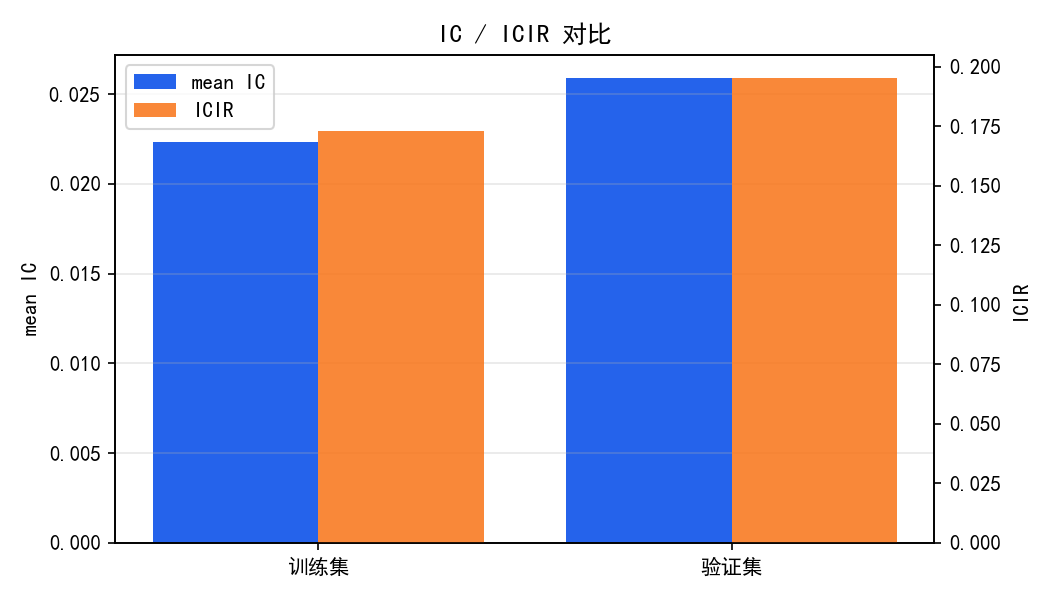
\includegraphics[width=0.82\textwidth]{fig2_ic_summary.png}
\caption{训练集与验证集 IC / ICIR 对比}
\label{fig:ic_bar}
\end{figure}

\begin{figure}[H]
\centering
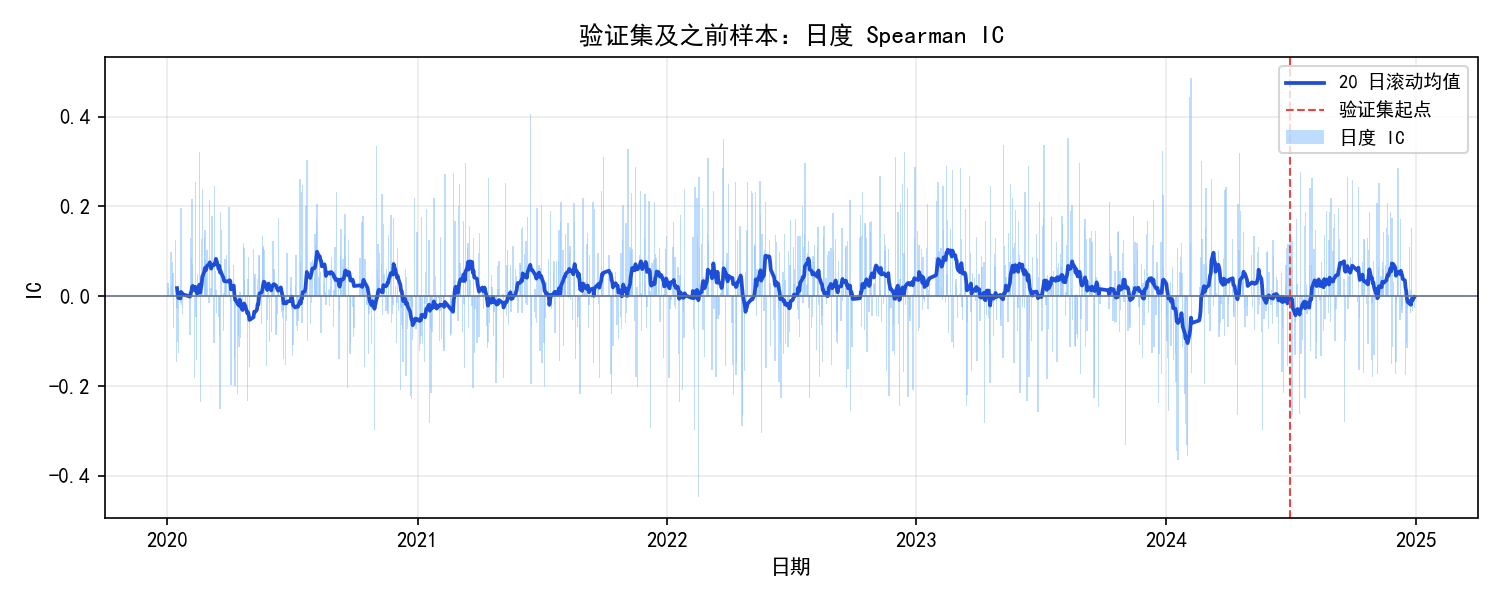
\includegraphics[width=\textwidth]{fig5_ic_timeseries.png}
\caption{日度 Spearman IC 及 20 日滚动均值（虚线为验证集起点 2024-07-01）}
\label{fig:ic_ts}
\end{figure}

\subsection{历史回测（验证集 2024 年下半年）}

\textbf{说明：}本实验无独立 test 集（数据止于 2024-12-31）。历史回测在\textbf{验证集}上进行，符合作业 PDF「测试集可划可不划，模拟比赛即为测试阶段」的要求。运行 \texttt{06\_backtest.py} 时 \texttt{test \{\}} 为空属预期：test 区间自 2025-01-01 起无交易日。

\begin{table}[H]
\centering
\caption{验证集历史回测结果（2024-07-01 --- 2024-12-31，124 个交易日）}
\label{tab:backtest}
\begin{tabular}{lrrl}
\toprule
\textbf{指标} & \textbf{本策略} & \textbf{沪深300} & \textbf{说明} \\
\midrule
初始资金     & \multicolumn{2}{c}{100 万元} & \\
总收益率 $R_{\mathrm{tot}}$     & \textbf{26.03\%} & 13.13\% & 区间实际收益 \\
复利年化 CAGR  & \textbf{60.01\%} & 28.50\% & $(P_T/P_0)^{252/n}-1$ \\
算术年化收益   & \textbf{54.32\%} & 28.51\% & $\bar{r}\times 252$，Sharpe 分子 \\
年化波动率     & 38.60\% & 26.44\% & $\mathrm{std}(r_t)\sqrt{252}$ \\
夏普比率       & \textbf{1.41} & 1.08 & $(\bar{r}\times 252)/\sigma_{\mathrm{ann}}$ \\
最大回撤 MDD   & \textbf{-15.53\%} & -10.99\% & \\
期末净值       & 126.03 万元 & 113.13 万元 & \\
\bottomrule
\end{tabular}
\end{table}

\textbf{数值解读：} 策略区间总收益 26\% 高于沪深 300 的 13\%，超额约 13 个百分点。夏普 1.41 $>$ 1.08，说明\textbf{单位风险下的收益}更好，但波动率也更高（38.6\% vs 26.4\%）。最大回撤 $-15.5\%$ 意味着从净值高点最多回落约 15.5\%。

验证集内策略表现优于基准，但样本仅约半年（124 日），统计显著性有限，不宜外推为长期表现。

\subsection{为什么 IC 很低（0.026），年化收益却很高（CAGR 60\%）？——初学者版}

这是阅读量化报告时最常见的困惑之一。下面用本实验\textbf{真实数字}分步说明，二者并不矛盾。

\paragraph{（1）IC 和「账户赚多少钱」本来就不是同一个指标}

\begin{itemize}[leftmargin=2em]
  \item \textbf{IC} 看的是：500 只股票全体上，分数与次日收益的相关性。IC$=0.026$ 表示「略好于瞎猜」，\textbf{不是}「预测很准」。
  \item \textbf{组合收益} 看的是：你实际买了哪几只、各买多少、扣费后净值涨了多少。
\end{itemize}

\textbf{类比：} IC 像「全班 500 人按预测成绩排名与真实成绩的相关性」；组合收益像「你只资助排名前 30 名，看他们整体表现如何」。全班相关性可以很低，但前 30 名仍可能明显强于后 30 名。

\paragraph{（2）策略只买头部，不看全市场 IC}

本策略 \texttt{q\_min=0.90}：只在 score 最高的 10\%（约 50 只）里选，最多持有 30 只。更相关的指标是\textbf{多空 spread}（完整公式与解读见附录~\ref{app:ic-vs-return}）：
\begin{equation}
  \mathrm{spread}_t
  = \bar{y}_{\mathrm{top\,10\%}} - \bar{y}_{\mathrm{bot\,10\%}},
  \qquad
  \overline{\mathrm{spread}} = 0.277\%\;/\;\text{日}
  \;\Rightarrow\;
  \text{年化 spread} \approx 69.8\%.
\end{equation}
即：高分组平均每日比低分组多赚 0.28\%（超额收益口径，未扣费）。这才是「头部是否跑赢尾部」的直接证据。验证集全市场 IC 仅 0.026，但 spread 显著为正——\textbf{分组有效}。

\paragraph{（3）Top 10\% 内的 IC 甚至为负，为什么还能赚钱？}

验证集 Top 10\% 内 IC $=-0.019$：在已经很好的 50 只股票里，再按分数细分，次序几乎随机。策略\textbf{不需要}在头部内部排得完美，只需要：
\begin{enumerate}[leftmargin=2em]
  \item 头部整体 $>$ 尾部整体（spread $>0$）；
  \item 把资金集中在头部（softmax 加权，非等权）。
\end{enumerate}

\paragraph{（4）「年化 60\%」主要来自短区间外推，不是 IC 直接换算来的}

验证集只有 124 个交易日（约半年），区间总收益 26.03\%。
\begin{itemize}[leftmargin=2em]
  \item \textbf{总收益 26\%}：半年实际赚到手的钱——最直观；
  \item \textbf{CAGR 60\%}：假设未来每半年都能复利 26\%，外推到整年——\textbf{headline 数字会偏大}；
  \item \textbf{算术年化 54\%}：日收益均值 $\times 252$，用于算 Sharpe。
\end{itemize}

若只看 CAGR 60\% 而不看「仅半年样本」，容易高估。报告同时列出总收益与两种年化，避免误读。

\paragraph{（5）spread 69.8\% $\neq$ 组合 26\%：中间还有策略与成本}

理论 spread（69.8\%）是「做多 top 10\%、做空 bottom 10\%」的\textbf{未扣费、未约束}参考；实际组合：
\begin{itemize}[leftmargin=2em]
  \item \textbf{只做多} Top 30，不做空；
  \item 单票/行业上限、现金 3\%、T+1、佣金印花税滑点；
  \item 整手交易、涨停买不到、换手限制 \texttt{omega\_max=25\%}。
\end{itemize}
因此实际总收益 26\% \textbf{低于} spread 暗示的上限，这是正常且健康的——说明回测没有简单把 spread 当收益。

\paragraph{（6）不是典型数据泄露}

若干预泄露，常见现象是训练 IC 虚高、验证 IC 崩掉。本实验训练 IC 0.022、验证 IC 0.026，接近且略升，更符合「轻度过拟合未发生」而非泄露。

\paragraph{（7）一句话总结}

\textbf{IC 低} = 全市场排序能力弱但为正；\textbf{收益高（相对基准）} = 头部相对尾部有 spread + 集中持仓 + 短区间 CAGR 外推放大。读报告时务必同时看：总收益、CAGR、算术年化、spread、样本长度。完整公式与数值对照见附录~\ref{app:ic-vs-return}。

\begin{figure}[H]
\centering
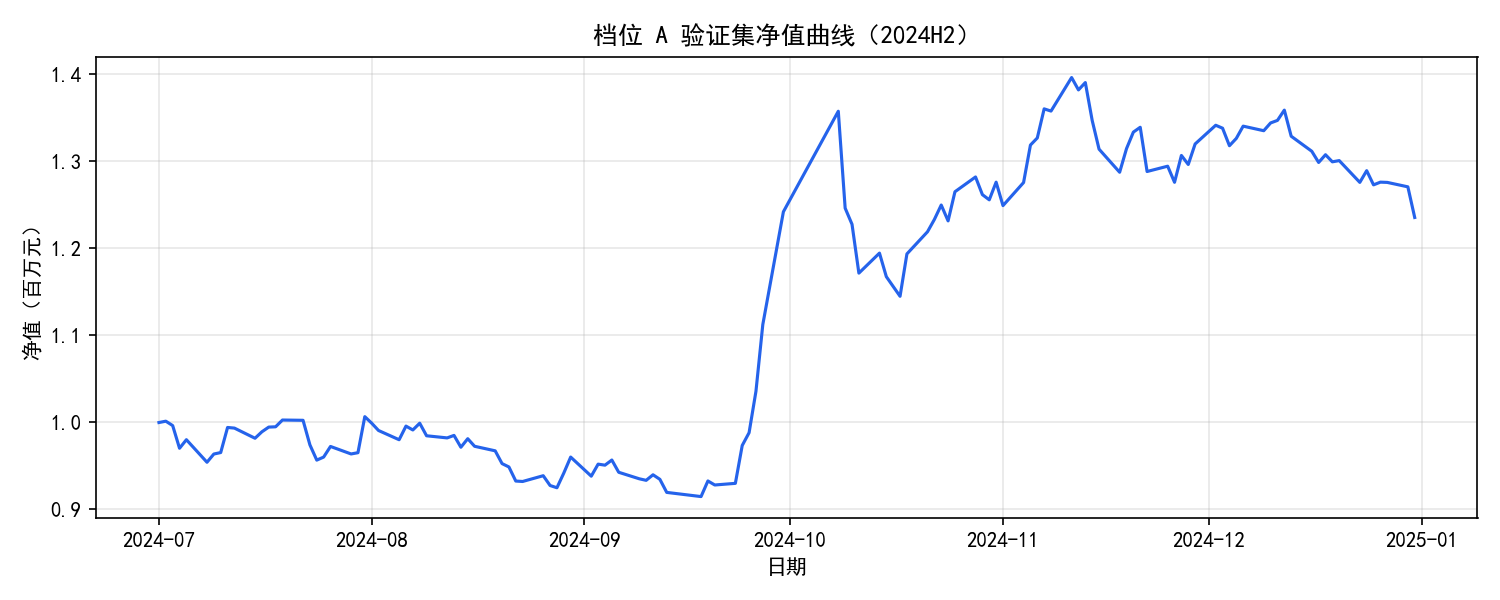
\includegraphics[width=\textwidth]{fig1_valid_equity.png}
\caption{验证集净值曲线（初始资金 100 万元）}
\label{fig:equity}
\end{figure}

验证集内策略收益与夏普高于沪深 300，但样本仅约半年，统计显著性有限，不宜外推为长期表现（详见上一节 IC 与收益关系分析）。

\subsection{融合权重与持仓分析}

\begin{figure}[H]
\centering
\begin{minipage}{0.46\textwidth}
  \centering
  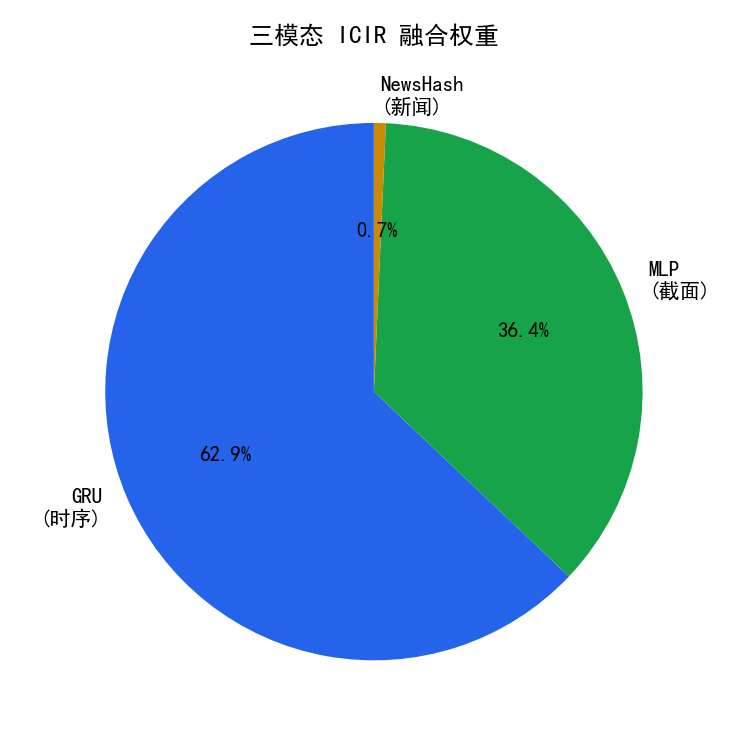
\includegraphics[width=\textwidth]{fig3_fusion_weights.png}
  \caption{三模态 ICIR 融合权重}
  \label{fig:fusion}
\end{minipage}\hfill
\begin{minipage}{0.52\textwidth}
  \centering
  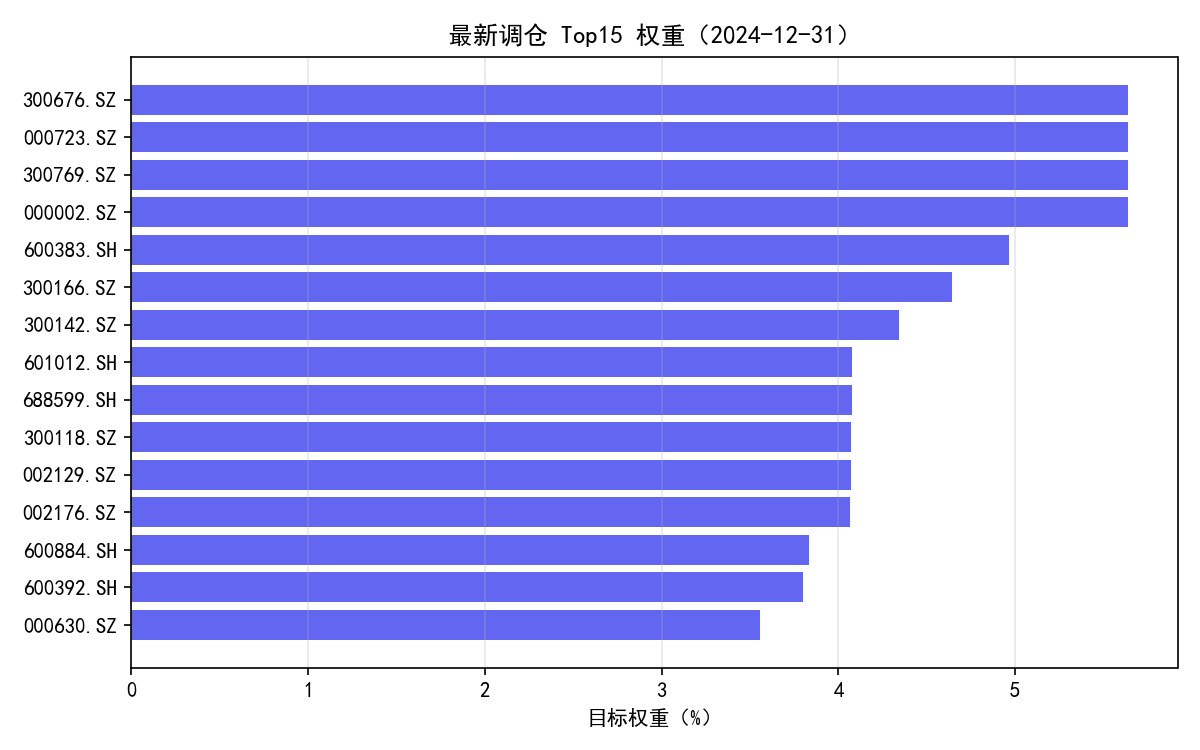
\includegraphics[width=\textwidth]{fig4_latest_orders.png}
  \caption{2024-12-31 最新调仓 Top15 目标权重}
  \label{fig:orders}
\end{minipage}
\end{figure}

\textbf{消融讨论：}
\begin{itemize}[leftmargin=2em]
  \item 新闻权重约 0.7\%：简单名称匹配 + 哈希难以捕捉语义，档位 C BERT-LoRA 可作对比；
  \item GRU 权重最高：价量时序是日频 alpha 主要来源；
  \item MLP 权重约 36\%：metric/moneyflow 提供增量信息。
\end{itemize}

%==============================================================================
\section{模拟交易与结果分析}
%==============================================================================

\subsection{比赛参与（赛后补全）}

正式比赛 FDL2026 时间为 2026-06-01 至 2026-06-12。本节在比赛结束后补充：
\begin{enumerate}[leftmargin=2em]
  \item 模拟账户收益趋势截图；
  \item 调仓记录与持仓记录截图；
  \item 模型分数与实际操作一致性说明；
  \item 比赛期间经验（成交困难、涨停、T+1 等）。
\end{enumerate}

\subsection{从模型到实盘的操作映射}

\begin{enumerate}[leftmargin=2em]
  \item 每个交易日收盘后更新数据，运行 \texttt{07\_predict\_latest.py}；
  \item 读取 \texttt{orders\_YYYYMMDD.csv} 中 \texttt{target\_weight}；
  \item 按账户总资产 $\times$ 权重计算目标市值，与当前持仓 diff 得到买卖清单；
  \item 次日交易时段委托；遵守 T+1 与尽可能满仓规则。
\end{enumerate}

%==============================================================================
\section{规范性与可复现性}
%==============================================================================

\begin{table}[H]
\centering
\caption{规则依从性检查}
\label{tab:compliance}
\begin{tabular}{lc}
\toprule
\textbf{检查项} & \textbf{状态} \\
\midrule
无未来信息泄露           & \checkmark \\
无全样本随机打乱         & \checkmark \\
流程含神经网络           & \checkmark \\
使用 metric/moneyflow/news 进阶数据 & \checkmark \\
尽可能满仓（权重和 $\approx$97\%） & \checkmark \\
T+1 可卖约束             & \checkmark \\
\bottomrule
\end{tabular}
\end{table}

\textbf{一键复现：}
\begin{verbatim}
conda activate ai25
cd code
python scripts/validate_tier_a_local.py
python scripts/run_tier_a_local.py
python ../tier_a_project/scripts/plot_tier_a_report.py
\end{verbatim}

依赖 \texttt{requirements.txt}（无需 NLP 包），预计耗时 1.5--3 小时（RTX 3060 6GB）。

%==============================================================================
\section{总结与反思}
%==============================================================================

\subsection{方案优点}

\begin{enumerate}[leftmargin=2em]
  \item \textbf{流程完整}：与课程 PDF 从数据到回测闭环一致，脚本模块化便于分工；
  \item \textbf{方法有依据}：GKX 预处理、IC 评估、多模态融合均有文献与业界对应；
  \item \textbf{可复现}：档位 A 在本机 6GB 显卡可稳定跑通；
  \item \textbf{防泄露意识}：逐日截面变换、新闻时间映射、walk-forward 切分均落实到代码。
\end{enumerate}

\subsection{局限性与改进方向}

\begin{table}[H]
\centering
\caption{局限性与后续改进}
\begin{tabular}{ll}
\toprule
\textbf{局限} & \textbf{改进方向} \\
\midrule
股票池仅 500 只     & 服务器档位 C：Top 3000 + 多 seed \\
新闻模态几乎无效   & RoBERTa-LoRA、事件分类 \\
验证期仅约半年     & 延长数据至 2025，增加 test 回测 \\
策略非 PDF 原始 Top-$k$ & 增加 Top-$k$ 消融对比 \\
\bottomrule
\end{tabular}
\end{table}

\subsection{个人感悟}

金融数据信噪比极低，训练 loss 下降慢、IC 绝对值小是常态，不应单纯追求回测高收益。预处理与标签构造与模型结构同样重要；一次全样本标准化就可能造成「虚假夏普」。预测分数到 PnL 之间还有组合构建与成本一层——\textbf{IC 衡量全市场排序，组合收益衡量实际持仓}，二者可能背离；读报告时应同时看 spread、总收益、CAGR 与样本长度。AI 辅助编码提高了效率，但数据对齐、shift 方向、T+1 等细节必须人工 review。

%==============================================================================
\section*{参考文献}
\addcontentsline{toc}{section}{参考文献}
%==============================================================================

\begin{enumerate}[leftmargin=2em]
  \item Gu, S., Kelly, B., \& Xiu, D. (2020). Empirical Asset Pricing via Machine Learning. \textit{Review of Financial Studies}.
  \item 课程讲义：《深度学习基础大作业.pdf》
  \item 《大作业评分细则.md》
  \item 项目组：《讨论报告.md》《项目方案.md》
  \item Fischer, T., \& Krauss, C. (2018). Deep learning with LSTM networks for financial market predictions. \textit{European Journal of Operational Research}.
\end{enumerate}

\appendix
\section{主要代码与产物路径}

\textbf{代码：}\texttt{code/config.tier\_a\_local.yaml}，\texttt{code/scripts/run\_tier\_a\_local.py}，\texttt{code/src/} 下各模块。

\textbf{产物：}
\begin{verbatim}
code/artifacts/metrics/tier_a/ic_summary.json
code/artifacts/backtest/tier_a/valid/metrics.json
code/artifacts/backtest/tier_a/valid/equity_curve.csv
code/artifacts/predictions/tier_a/fusion_weights.json
code/artifacts/orders/tier_a/orders_20241231.csv
\end{verbatim}

\textbf{报告图表：}\texttt{tier\_a\_project/figures/fig1\_valid\_equity.png} 等五张图。

\section{附录 B：为什么 IC 很低，年化收益却很高？（初学者完整版）}
\label{app:ic-vs-return}

阅读本报告时，最容易产生的疑问是：验证集 \textbf{mean IC 只有 0.026}（几乎接近 0），但回测 \textbf{CAGR 却显示 60\%}——是不是算错了？是不是数据泄露？本节用\textbf{标准公式 + 本实验真实数字}完整说明：二者衡量的是\textbf{不同问题}，并不矛盾。

\subsection{先记住：IC 和「账户赚多少钱」不是同一个指标}

\paragraph{IC 的定义与意义}

对每个交易日 $t$，在当日股票横截面上计算 Spearman 秩相关：
\begin{equation}
  \mathrm{IC}_t = \mathrm{Spearman}\big(\{s_{i,t}\},\ \{y_{i,t}\}\big),
  \qquad
  \overline{\mathrm{IC}} = \frac{1}{D}\sum_{t=1}^{D}\mathrm{IC}_t.
\end{equation}
其中 $s_{i,t}$ 为模型分数，$y_{i,t}$ 为次日相对沪深 300 的超额收益，$D$ 为有效交易日数。

\textbf{实际意义：} IC 回答「\textbf{全体股票}里，分高的明天是否涨得多」。本实验验证集 $\overline{\mathrm{IC}}=0.0259$：
\begin{itemize}[leftmargin=2em]
  \item 不是「预测准确率 2.6\%」，而是\textbf{排序与收益的秩相关}约为 0.026；
  \item 0 表示和瞎猜一样；0.02--0.05 在日频 A 股里属\textbf{常见可用}区间；不必期待 IC 接近 1。
\end{itemize}

\paragraph{组合收益的定义与意义}

回测看的是净值曲线 $P_t$ 及：
\begin{equation}
  R_{\mathrm{tot}} = \frac{P_T}{P_0}-1,
  \qquad
  \mathrm{CAGR} = \left(\frac{P_T}{P_0}\right)^{252/n}-1,
  \qquad
  \bar{r}\times 252 \;\text{（算术年化，Sharpe 分子）}.
\end{equation}

\textbf{实际意义：} 组合收益回答「\textbf{实际买了哪些股票、各买多少、扣费后}净值涨了多少」。

\paragraph{类比（帮助直觉）}

\begin{itemize}[leftmargin=2em]
  \item \textbf{IC}：像「全班 500 人，按预测成绩排名与真实成绩的相关性」——可以很低；
  \item \textbf{组合收益}：像「你只资助排名前 30 名，看他们整体表现」——前 30 名仍可能明显强于后 30 名。
\end{itemize}

\subsection{策略实际在做什么？——因此不能只看全市场 IC}

本策略 \texttt{q\_min=0.90}，\texttt{n\_max=30}：
\begin{enumerate}[leftmargin=2em]
  \item 只在当日 score 位于\textbf{最高 10\%}的股票（约 50 只）里选；
  \item 最多持有\textbf{30 只}，按分数 softmax 加权（非等权）；
  \item 不做空，留约 3\% 现金，并受单票/行业上限、T+1、交易成本等约束。
\end{enumerate}

因此更该问：\textbf{「头部是否跑赢尾部？」} 而不是「500 只全体排得多准？」

\subsection{更贴近策略的指标：多空 spread}

\paragraph{公式（标准定义）}

对每个交易日 $t$，记 $y_{i,t}$ 为股票 $i$ 的次日超额收益，按 score 划分：
\begin{itemize}[leftmargin=2em]
  \item $\mathcal{T}_t$：score 位于当日最高 10\% 分位及以上的股票集合（top）；
  \item $\mathcal{B}_t$：score 位于当日最低 10\% 分位及以下的股票集合（bottom）。
\end{itemize}
日度多空 spread 定义为
\begin{equation}
  \mathrm{spread}_t
  = \bar{y}_{\mathrm{top\,10\%},\,t} - \bar{y}_{\mathrm{bot\,10\%},\,t}
  = \frac{1}{|\mathcal{T}_t|}\sum_{i\in\mathcal{T}_t} y_{i,t}
   - \frac{1}{|\mathcal{B}_t|}\sum_{i\in\mathcal{B}_t} y_{i,t}.
  \label{eq:spread-daily}
\end{equation}
对 $D$ 个交易日求平均并年化：
\begin{equation}
  \overline{\mathrm{spread}} = \frac{1}{D}\sum_{t=1}^{D}\mathrm{spread}_t,
  \qquad
  \text{年化 spread} = \overline{\mathrm{spread}} \times 252.
  \label{eq:spread-ann}
\end{equation}

\paragraph{本实验验证集实际数值}

\begin{center}
\begin{tabular}{lrl}
\toprule
\textbf{指标} & \textbf{数值} & \textbf{含义} \\
\midrule
全市场 mean IC & 0.0259 & 500 只全体排序略优于随机 \\
Top 10\% 内 mean IC & $-0.0192$ & 头部 50 只\textbf{内部}再排序，噪声大 \\
日均 spread & 0.277\% & 高分组日均多赚 0.28 个百分点 \\
年化 spread & 69.8\% & 式~(\ref{eq:spread-ann})，\textbf{未扣费、未约束} \\
\bottomrule
\end{tabular}
\end{center}

\textbf{解读：} 全市场 IC 仅 0.026，但 spread 显著为正——说明\textbf{分组有效}（头部整体 $>$ 尾部整体），这才是「只买头部」策略更该看的证据。

\subsection{Top 10\% 内 IC 为负，为什么还能赚钱？}

验证集 Top 10\% 内 IC $=-0.019$：在已经很好的约 50 只股票里，再按分数细分，次序几乎随机。

策略\textbf{不需要}在头部内部排得完美，只需要：
\begin{enumerate}[leftmargin=2em]
  \item 头部整体优于尾部整体（spread $>0$，本实验成立）；
  \item 把资金集中在头部（softmax 加权，非等权）。
\end{enumerate}

\subsection{「年化 60\%」从哪来？——不是 IC 直接换算的}

验证集仅 \textbf{124 个交易日}（约半年）。本实验回测数字：

\begin{center}
\begin{tabular}{lrr}
\toprule
\textbf{指标} & \textbf{本策略} & \textbf{说明} \\
\midrule
区间总收益 $R_{\mathrm{tot}}$ & \textbf{26.03\%} & 半年\textbf{实际}赚到手的钱 \\
复利年化 CAGR & \textbf{60.01\%} & $(1.2603)^{252/124}-1$，外推整年 \\
算术年化 $\bar{r}\times 252$ & \textbf{54.32\%} & Sharpe 分子 \\
夏普比率 & 1.41 & 同期沪深 300 为 1.08 \\
\bottomrule
\end{tabular}
\end{center}

\textbf{初学者易错点：}
\begin{itemize}[leftmargin=2em]
  \item 看到「年化 60\%」$\neq$ 半年赚了 60\%——\textbf{实际总收益是 26\%}；
  \item CAGR 是把半年收益复利外推到整年的 headline 数字，短样本会\textbf{放大}观感；
  \item 报告同时列出总收益、CAGR、算术年化，避免只读一个数。
\end{itemize}

\subsection{spread 69.8\% $\neq$ 组合 26\%：中间还有策略层与成本}

式~(\ref{eq:spread-ann}) 的 69.8\% 是「做多 top 10\%、做空 bottom 10\%」的\textbf{理论参考}（未扣费、无 A 股约束）。实际组合还有：

\begin{itemize}[leftmargin=2em]
  \item \textbf{只做多} Top 30，不做空；
  \item 佣金 0.015\%、卖出印花税 0.05\%、滑点 0.05\%；
  \item T+1、100 股整手、涨停买不到；
  \item 单票上限 5\%、行业上限 25\%、现金 3\%、单日换手上限 25\%。
\end{itemize}

因此实际总收益 26\% \textbf{低于} spread 暗示的上限——这是正常且健康的，说明回测没有简单把 spread 当组合收益。

\subsection{是不是数据泄露或公式算错？}

\textbf{不太像典型泄露：} 训练 IC $=0.022$，验证 IC $=0.026$，接近且略升；若干预泄露，常见 pattern 是训练 IC 虚高、验证 IC 崩掉。

\textbf{公式已按标准修正：} 夏普用 $(\bar{r}\times 252)/\sigma_{\mathrm{ann}}$，不再误用 $\mathrm{CAGR}/\sigma$；CAGR 与算术年化分开报告（见正文表~\ref{tab:metric-def}、表~\ref{tab:backtest}）。

\subsection{读报告时建议对照的检查清单}

\begin{enumerate}[leftmargin=2em]
  \item 全市场 IC 多少？（本实验 0.026，弱但为正）
  \item spread 是否为正？（本实验日均 0.277\%，是）
  \item 区间总收益多少？（本实验 26\%，最直观）
  \item CAGR 与算术年化是否分开读？（60\% vs 54\%）
  \item 样本多长？（124 日，约半年，不宜外推）
  \item 相对基准如何？（沪深 300 总收益 13\%，Sharpe 1.08 $<$ 1.41）
\end{enumerate}

\subsection{一句话总结}

\textbf{IC 低}（0.026）$=$ 全市场 500 只排序能力弱但为正；\textbf{收益相对较高}（总收益 26\%，CAGR 60\% 为短样本外推）$=$ 头部相对尾部有 spread + 集中持仓 + 扣费后仍跑赢基准。\;二者\textbf{不矛盾}，因为问的问题不同。

\end{document}
